%%%%%%%%%%%%%%%%%%%%%%%%%%%%%%%%%%%%%%%%%
% Beamer Presentation
% LaTeX Template
% Version 1.0 (10/11/12)
%
% This template has been downloaded from:
% http://www.LaTeXTemplates.com
%
% License:
% CC BY-NC-SA 3.0 (http://creativecommons.org/licenses/by-nc-sa/3.0/)
%
%%%%%%%%%%%%%%%%%%%%%%%%%%%%%%%%%%%%%%%%%

%----------------------------------------------------------------------------------------
%	PACKAGES AND THEMES
%----------------------------------------------------------------------------------------

%\documentclass{beamer}
\documentclass[12pt, aspectratio=169]{beamer}
\usepackage{keynote-gradient}

\mode<presentation> {

% The Beamer class comes with a number of default slide themes
% which change the colors and layouts of slides. Below this is a list
% of all the themes, uncomment each in turn to see what they look like.

%\usetheme{default}
%\usetheme{AnnArbor}
%\usetheme{Antibes}
%\usetheme{Bergen}
%\usetheme{Berkeley}
%\usetheme{Berlin}
%\usetheme{Boadilla}
%\usetheme{CambridgeUS}
%\usetheme{Copenhagen}
%\usetheme{Darmstadt}
%\usetheme{Dresden}
%\usetheme{Frankfurt}
%\usetheme{Goettingen}
%\usetheme{Hannover}
%\usetheme{Ilmenau}
%\usetheme{JuanLesPins}
%\usetheme{Luebeck}
%\usetheme{Madrid}
%\usetheme{Malmoe}
%\usetheme{Marburg}
%\usetheme{Montpellier}
%\usetheme{PaloAlto}
%\usetheme{Pittsburgh}
%\usetheme{Rochester}
%\usetheme{Singapore}
%\usetheme{Szeged}
%\usetheme{Warsaw}

% As well as themes, the Beamer class has a number of color themes
% for any slide theme. Uncomment each of these in turn to see how it
% changes the colors of your current slide theme.

%\usecolortheme{albatross}
%\usecolortheme{beaver}
%\usecolortheme{beetle}
%\usecolortheme{crane}
%\usecolortheme{dolphin}
%\usecolortheme{dove}
%\usecolortheme{fly}
%\usecolortheme{lily}
%\usecolortheme{orchid}
%\usecolortheme{rose}
%\usecolortheme{seagull}
%\usecolortheme{seahorse}
%\usecolortheme{whale}
%\usecolortheme{wolverine}

%\setbeamertemplate{footline} % To remove the footer line in all slides uncomment this line
\setbeamertemplate{footline}[page number] % To replace the footer line in all slides with a simple slide count uncomment this line

\setbeamertemplate{navigation symbols}{} % To remove the navigation symbols from the bottom of all slides uncomment this line
}

\usepackage{graphicx} % Allows including images
\usepackage{booktabs} % Allows the use of \toprule, \midrule and \bottomrule in tables

%----------------------------------------------------------------------------------------
%	TITLE PAGE
%----------------------------------------------------------------------------------------

\title[AI intro]{AI introduction \\elective} % The short title appears at the bottom of every slide, the full title is only on the title page

\author[Max Talanov, Alexander Kirilovich]{
  
\includegraphics[height=3cm]{ITIS_logo_bright}\\
  Max Talanov, Alexander Kirilovich
} 
\institute[ITIS: KFU] % Your institution as it will appear on the bottom of every slide, may be shorthand to save space
{
Machine cognition lab, Intellectual robotics department, ITIS \\ % Your institution for the title page
\medskip
\textit{max.talanov@gmail.com} % Your email address
}
\date{\today} % Date, can be changed to a custom date

\begin{document}

\begin{frame}
\titlepage % Print the title page as the first slide
\end{frame}


%----------------------------------------------------------------------------------------
%	PRESENTATION SLIDES
%----------------------------------------------------------------------------------------

%------------------------------------------------
\section{Main achievements of AI} % Sections can be created in order to organize your presentation into discrete blocks, all sections and subsections are automatically printed in the table of contents as an overview of the talk
%------------------------------------------------
%------------------------------------------------
\begin{frame}
\frametitle{Main players in AI}
\begin{figure}
  
\includegraphics[width=0.45\linewidth]{220px-IBM.png}
  
\includegraphics[width=0.45\linewidth]{220px-Microsoft.png}
\end{figure}
\begin{figure}
  
\includegraphics[width=0.45\linewidth]{220px-Google.png}
  
\includegraphics[width=0.45\linewidth]{220px-Facebook.png}
\end{figure}
\end{frame}
%------------------------------------------------
%------------------------------------------------
\begin{frame}
\frametitle{Kasparov vs Deep Blue}
\begin{columns}[c]
\column{.5\textwidth} % Left column and width
\begin{figure}
  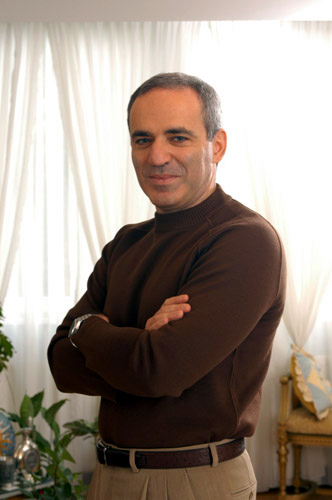
\includegraphics[width=1\linewidth]{Kasparov-34.jpg}
\end{figure}
\column{.5\textwidth} % Left column and width
\begin{figure}
  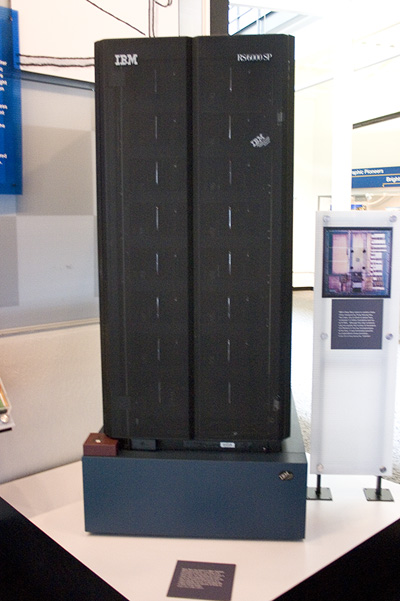
\includegraphics[width=1\linewidth]{Deep_Blue.jpg}
\end{figure}
\end{columns}
\end{frame}
%------------------------------------------------
%------------------------------------------------
\begin{frame}
\frametitle{Watson in Jeopardy}
\begin{columns}[c]
\column{.5\textwidth} % Left column and width
\begin{figure}
  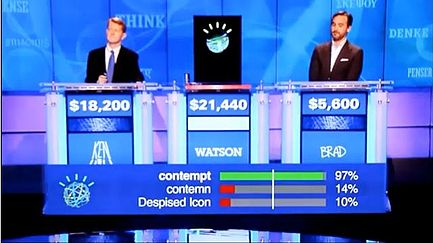
\includegraphics[width=1\linewidth]{Watson_Jeopardy.jpg}
\end{figure}
\column{.5\textwidth} % Left column and width
\begin{figure}
  
\includegraphics[width=1\linewidth]{Watson's_avatar.jpg}
\end{figure}
\end{columns}
\end{frame}
%------------------------------------------------
%------------------------------------------------
\begin{frame}
\frametitle{AlphaGo}
\begin{figure}
  
\includegraphics[width=0.45\linewidth]{220px-Alphago.png}
\end{figure}
\begin{figure}
  
\includegraphics[width=0.45\linewidth]{DeepMind_logo.png}
\end{figure}
\end{frame}
%------------------------------------------------
%------------------------------------------------
\begin{frame}
\frametitle{Main topics}
\begin{itemize}
\item Big Data
\item Machine learning
\item Decision making
\item Knowledge management
\item Semantic networks
\item Neural networks
\end{itemize}
\end{frame}
%------------------------------------------------
%------------------------------------------------
\begin{frame}
\frametitle{Main technologies and tools}
\begin{itemize}
\item Rapid miner
\item Weka
\item OWL
\item Protege
\item NARS
\item \ldots
\end{itemize}
\end{frame}
%------------------------------------------------
%------------------------------------------------

\end{document} 
